% Options for packages loaded elsewhere
\PassOptionsToPackage{unicode}{hyperref}
\PassOptionsToPackage{hyphens}{url}
%
\documentclass[
  12pt,
  a4paperpaper,
]{report}
\usepackage{lmodern}
\usepackage{amssymb,amsmath}
\usepackage{ifxetex,ifluatex}
\ifnum 0\ifxetex 1\fi\ifluatex 1\fi=0 % if pdftex
  \usepackage[T1]{fontenc}
  \usepackage[utf8]{inputenc}
  \usepackage{textcomp} % provide euro and other symbols
\else % if luatex or xetex
  \usepackage{unicode-math}
  \defaultfontfeatures{Scale=MatchLowercase}
  \defaultfontfeatures[\rmfamily]{Ligatures=TeX,Scale=1}
\fi
% Use upquote if available, for straight quotes in verbatim environments
\IfFileExists{upquote.sty}{\usepackage{upquote}}{}
\IfFileExists{microtype.sty}{% use microtype if available
  \usepackage[]{microtype}
  \UseMicrotypeSet[protrusion]{basicmath} % disable protrusion for tt fonts
}{}
\makeatletter
\@ifundefined{KOMAClassName}{% if non-KOMA class
  \IfFileExists{parskip.sty}{%
    \usepackage{parskip}
  }{% else
    \setlength{\parindent}{0pt}
    \setlength{\parskip}{6pt plus 2pt minus 1pt}}
}{% if KOMA class
  \KOMAoptions{parskip=half}}
\makeatother
\usepackage{xcolor}
\IfFileExists{xurl.sty}{\usepackage{xurl}}{} % add URL line breaks if available
\IfFileExists{bookmark.sty}{\usepackage{bookmark}}{\usepackage{hyperref}}
\hypersetup{
  hidelinks,
  pdfcreator={LaTeX via pandoc}}
\urlstyle{same} % disable monospaced font for URLs
\usepackage{graphicx}
\makeatletter
\def\maxwidth{\ifdim\Gin@nat@width>\linewidth\linewidth\else\Gin@nat@width\fi}
\def\maxheight{\ifdim\Gin@nat@height>\textheight\textheight\else\Gin@nat@height\fi}
\makeatother
% Scale images if necessary, so that they will not overflow the page
% margins by default, and it is still possible to overwrite the defaults
% using explicit options in \includegraphics[width, height, ...]{}
\setkeys{Gin}{width=\maxwidth,height=\maxheight,keepaspectratio}
% Set default figure placement to htbp
\makeatletter
\def\fps@figure{htbp}
\makeatother
\setlength{\emergencystretch}{3em} % prevent overfull lines
\providecommand{\tightlist}{%
  \setlength{\itemsep}{0pt}\setlength{\parskip}{0pt}}
\setcounter{secnumdepth}{5}



% Table of contents formatting
\renewcommand{\contentsname}{Table of Contents}
\setcounter{tocdepth}{3}

% Headers and page numbering
\usepackage{fancyhdr}
\pagestyle{plain}

% Following package is used to add background image to front page
\usepackage{wallpaper}

% interleave pdfs into final document
\usepackage{pdfpages}

% Table package
\usepackage{ctable}% http://ctan.org/pkg/ctable

% Deal with 'LaTeX Error: Too many unprocessed floats.'
\usepackage{morefloats}
% or use \extrafloats{100}
% add some \clearpage

% % Chapter header
% \usepackage{titlesec, blindtext, color}
% \definecolor{gray75}{gray}{0.75}
% \newcommand{\hsp}{\hspace{20pt}}
% \titleformat{\chapter}[hang]{\Huge\bfseries}{\thechapter\hsp\textcolor{gray75}{|}\hsp}{0pt}{\Huge\bfseries}

% % Fonts and typesetting
% \setmainfont[Scale=1.1]{Helvetica}
% \setsansfont[Scale=1.1]{Verdana}

% FONTS
\usepackage{xunicode}
\usepackage{xltxtra}
\defaultfontfeatures{Mapping=tex-text} % converts LaTeX specials (``quotes'' --- dashes etc.) to unicode
% \setromanfont[Scale=1.01,Ligatures={Common},Numbers={OldStyle}]{Palatino}
% \setromanfont[Scale=1.01,Ligatures={Common},Numbers={OldStyle}]{Adobe Caslon Pro}
%Following line controls size of code chunks
% \setmonofont[Scale=0.9]{Monaco}
%Following line controls size of figure legends
% \setsansfont[Scale=1.2]{Optima Regular}

%Attempt to set math size
%First size must match the text size in the document or command will not work
%\DeclareMathSizes{display size}{text size}{script size}{scriptscript size}.
\DeclareMathSizes{12}{13}{7}{7}

% ---- CUSTOM AMPERSAND
% \newcommand{\amper}{{\fontspec[Scale=.95]{Adobe Caslon Pro}\selectfont\itshape\&}}

% HEADINGS
\usepackage{sectsty}
\usepackage[normalem]{ulem}
\sectionfont{\rmfamily\mdseries\Large}
\subsectionfont{\rmfamily\mdseries\scshape\large}
\subsubsectionfont{\rmfamily\bfseries\upshape\large}
% \sectionfont{\rmfamily\mdseries\Large}
% \subsectionfont{\rmfamily\mdseries\scshape\normalsize}
% \subsubsectionfont{\rmfamily\bfseries\upshape\normalsize}

% Set figure legends and captions to be smaller sized sans serif font
\usepackage[font={footnotesize,sf}]{caption}

\usepackage{siunitx}

% Adjust spacing between lines to 1.5
\usepackage{setspace}
\onehalfspacing
% \doublespacing
\raggedbottom

% Set margins
\usepackage[top=1.1in,bottom=1.1in,left=1.5in,right=1.4in]{geometry}
% \setlength\parindent{0.4in} % indent at start of paragraphs (set to 0.3?)
\setlength{\parskip}{9pt}

% Add space between pararaphs
% http://texblog.org/2012/11/07/correctly-typesetting-paragraphs-in-latex/
% \usepackage{parskip}
% \setlength{\parskip}{\baselineskip}

% Set colour of links to black so that they don't show up when printed
\usepackage{hyperref}
\hypersetup{colorlinks=false, linkcolor=black}

% Tables
\usepackage{booktabs}
\usepackage{threeparttable}
\usepackage{array}
\newcolumntype{x}[1]{%
>{\centering\arraybackslash}m{#1}}%

% Allow for long captions and float captions on opposite page of figures
% \usepackage[rightFloats, CaptionBefore]{fltpage}

% Don't let floats cross subsections
% \usepackage[section,subsection]{extraplaceins}


\author{}
\date{}

\begin{document}

\hypertarget{general-introduction}{%
\chapter{General introduction}\label{general-introduction}}

\hypertarget{the-role-of-clinical-chemistry-in-medicine}{%
\section{The role of clinical chemistry in
medicine}\label{the-role-of-clinical-chemistry-in-medicine}}

Medicine is an art and a science in the service of fellow human beings
{[}1{]}. On the basis of collected empirical data and information,
clinicians select specific diagnoses, rule out other differential
diagnoses and eventually make decisions about which and how specific
therapeutic interventions are made for the benefit and health of their
patients. For a proper interpretation, collected data and information
must be compared with other, already existing, data and information to
assess the exact value of the clinician's findings. Moreover, a
clinician compares observed medical data of a patient with knowledge
obtained during his or her training as a clinician and with the
experience obtained by working with other patients.

A prerequisite in this paradigm, however, is that collected empirical
data on which the diagnoses of a clinician are based must be as
objective as possible. Clinical chemistry takes a pivotal role in this
in the sense that the chemical characterisation of a patient's body
fluid is one of the ways in medicine that can provide such objective
data. Since the beginning of this century, clinical chemistry has
evolved into a separate and independent discipline in the field of
medicine {[}2-4{]}. Nowadays, most often a single central clinical
chemistry laboratory takes care of the `analytical needs' of one or more
hospitals.

Tasks of the clinical chemist typically include the improvement of
existing methods of chemical analysis, the development of new analytical
methods and providing the clinician with as much information as possible
on the basis of chemical analyses. Especially this last task forms the
basis of what has become known as \emph{chemometrics}, a branch of
clinical chemistry that uses mathematical and statistical methods to
extract a maximum of information from chemical analyses {[}5, 6{]}.

This thesis presents a multivariate chemometric approach to the problems
that are currently associated with the interpretation and evaluation of
those laboratory measurements that are used to assess the arterial
acid-base status of a patient in an intensive care unit (ICU).

\hypertarget{arterial-acid-base-measurements-in-the-icu}{%
\section{Arterial acid-base measurements in the
ICU}\label{arterial-acid-base-measurements-in-the-icu}}

The ICU of today is a highly specialised ward in which expert medical,
nursing and technical staff provides medical services to severely ill
patients. It is characterised as a high-tech environment in which the
real-time monitoring of vital functions plays a central role. The origin
of the ICU can be traced back to the second half of the
19\textsuperscript{th} century when special rooms, adjacent to the
operating room, were used primarily for the purpose of postoperative
care {[}7{]}. In the course of time, these recovery rooms evolved into
specialised respiratory care units and shock and trauma units,
eventually leading to the present day ICU. The modern ICU provides
integrated cardiopulmonary support for both medical and surgical
patients suffering from severe respiratory and / or cardiac problems as
a result of disease or trauma.

The most frequently ordered chemical test in the ICU is the arterial
blood gas measurement {[}8{]}. Arterial blood gas measurements comprise
those measurements of the patient's arterial blood that are used for the
evaluation and interpretation of the patient's oxygen and acid-base
status. Basic arterial blood gas measurements include: the partial
pressure of oxygen (PaO\textsubscript{2}), the oxygen saturation of
haemoglobin, the pH of arterial blood, the partial pressure of carbon
dioxide (\(\ce{PaCO}_{2}\)) and the bicarbonate-ion concentration
(a{[}\(\text{HCO}_{3}^{-}\){]}). The first two measurements
(PaO\textsubscript{2} and oxygen saturation) are used to evaluate the
oxygen status, while the other three are used for the interpretation of
the arterial acid-base status.

In a strict sense, the term blood gas measurements is incorrect, since
only PaO\textsubscript{2} and \(\ce{PaCO}_{2}\) are true gas
measurements and in modern chemical analysers
a{[}\(\text{HCO}_{3}^{-}\){]} is not measured but calculated from
measured pH and \(\ce{PaCO}_{2}\). Moreover, two other derived acid-base
parameters are generally considered part of the set of arterial blood
gas measurements. These parameters are the standard bicarbonate-ion
concentration (SB) and the base excess (BE). Their derivation and
rationale are described in section 1.4.3 in more detail.

Since the second half of this century, the analysis of arterial blood
for the purpose of acid-base characterisation has become a vital part of
intensive care medicine. The importance of the acid-base
characterisation of arterial blood is illustrated by the severe polio
epidemic that struck Copenhagen (Denmark) in 1952 {[}9{]}. During this
epidemic, hospitals in Copenhagen had to cope with a large number of
patients needing intensive artificial respiration as a result of
paralysis of the respiratory muscles. For a proper setting of the
artificial respiration, the complete acid-base status of the patient had
to be known. At that time, arterial blood of patients was seldom sampled
for the purpose of performing blood gas measurements {[}10{]}. Arterial
blood gas measurements were mainly performed in physiological
laboratories and were not part of daily clinical practice. Techniques of
measurement were cumbersome and needed large equipment.

The clinical necessity of quickly knowing the patient's arterial
acid-base status for the purpose of a proper adjustment of the
artificial respiration inspired Poul Astrup to develop his equilibration
method {[}9{]}. This method allowed a relatively quick determination of
the three basic acid-base parameters by only measuring the pH of an
arterial blood sample and the pH of the sample equilibrated at two known
\(\ce{PaCO}_{2}\) gas tensions. The original PaCO­\textsubscript{2} is
calculated by interpolation {[}11, 12{]}. Since then, techniques of
analysis developed and arterial acid-base measurements have become
routine and indispensable in the daily clinical care of intensive care
patients.

\hypertarget{basic-acid-base-physiology}{%
\section{Basic acid-base physiology}\label{basic-acid-base-physiology}}

In chemical terms, acids are substances that are capable of donating
hydrogen (\(H^{+}\)) ions while bases are substances capable of
accepting \(H^{+}\) ions. The amount of \(H^{+}\) ions in the arterial
blood determines its actual acidity. Acidity is measured as pH, which
is, according to the definition of Sörensen, the negative logarithm of
the \(H^{+}\) concentration ({[}\(H^{+}\){]}) {[}9{]}.

The regulation of the amount of \(H^{+}\) ions in the arterial blood and
consequently its pH is one of the most powerful controlling mechanisms
in the human body. Under normal physiologic conditions, the pH of
arterial blood is kept within well-defined limits. This tight regulation
of the \(H^{+}\) concentration in arterial blood is essential since
\(H^{+}\) ions are highly reactive with negatively charged parts of
molecules. Changes in \(H^{+}\) concentration (intra-cellular as well as
extra-cellular) therefore have a profound influence on the molecular
configuration and consequently on protein function {[}13{]}. Hence,
maintaining a constant pH ensures an optimal working condition for
enzymes and other proteins. Moreover, large deviations in pH may have
effects on the nervous system. If the body becomes too acidic, the
nervous system can become so depressed that death can occur. On the
other hand, if the body becomes too alkaline, the nervous system can
become overexcited, resulting in death from tetanus of the respiratory
muscle {[}14{]}.

Two mechanisms exist to regulate pH of arterial blood: long term
physiological buffering and short term chemical buffering. Physiological
buffering is the redistribution, production, excretion and/or retention
of (non-)volatile acids and bases by means of physiological processes.
Chemical buffering is the result of the presence of weak acids and their
conjugated bases in the arterial blood. Examples of chemical buffers in
arterial blood are: inorganic phosphate, organic phosphate and
haemoglobin.

One of the most important chemical buffer systems in the blood, however,
is the bicarbonate ion (\(\text{HCO}_{3}^{-}\))/carbon dioxide
(\(\ce{CO}_{2}\)) buffer system. It is mainly the presence of this
buffer system that makes it possible for the human body to cope with the
constant load of exogenous acids and bases and the vast amount of both
volatile and non-volatile acids that are continuously generated as a
result of normal metabolism.

The equation describing the \(\text{HCO}_{3}^{-}\)/\(\ce{CO}_{2}\)
buffer system in blood is:

\(\text{CO}_{2} + H_{2}O \Leftrightarrow H_{2}\text{CO}_{3} \Leftrightarrow H^{+} + \text{HCO}_{3}^{-}\)
(1--1)

The left-hand side of this chemical reaction represents the formation of
carbonic acid (H\textsubscript{2}CO\textsubscript{3}) from
\(\ce{CO}_{2}\) and H\textsubscript{2}O. Therefore, although
\(\ce{CO}_{2}\) itself is not an acid, an elevation of the
\(\ce{CO}_{2}\) in the blood increases the acidity of the blood through
the formation of H\textsubscript{2}CO\textsubscript{3} which immediately
dissociates into protons (\(H^{+}\)) and bicarbonate ions
(\(\text{HCO}_{3}^{-}\)).

Since the concentration of H\textsubscript{2}CO\textsubscript{3} is so
low in relation to the concentration of dissolved \(\ce{CO}_{2}\) and
the concentration of \(\text{HCO}_{3}^{-}\), the law of mass action for
the \(\text{HCO}_{3}^{-}\)/\(\ce{CO}_{2}\) buffer system is:

\(K = \frac{\left\lbrack H^{+} \right\rbrack \times \left\lbrack \text{HCO}_{3}^{-} \right\rbrack}{\left\lbrack \text{CO}_{2} \right\rbrack \times \left\lbrack H_{2}O \right\rbrack}\),
(1--2)

where K is a constant.

Because {[}H\textsubscript{2}O{]} is relatively constant in body fluids,
it can be omitted from the equation and incorporated into the constant
K, further indicated as K' {[}13{]}. Rewriting the resulting equation to
solve {[}\(H^{+}\){]} yields the equation that Lawrence Joseph Henderson
(1878-1942) first described in 1909 {[}10{]}:

\(\left\lbrack H^{+} \right\rbrack = K^{'} \times \frac{\left\lbrack \text{CO}_{2} \right\rbrack}{\left\lbrack \text{HCO}_{3}^{-} \right\rbrack}\)
(1--3)

The concentration of dissolved \(\ce{CO}_{2}\) in blood
({[}\(\ce{CO}_{2}\){]}) is proportional to the partial pressure of
\(\ce{CO}_{2}\) (PCO\textsubscript{2}) in the gas with which the blood
is in equilibrium. Therefore, {[}\(\ce{CO}_{2}\){]} can be replaced by
the partial pressure of \(\ce{CO}_{2}\) in the blood. Partial pressures
are either measured in millimetres mercury (mmHg) or kilo-Pascal (kPa)
where 1 mmHg = 0.133 kPa. The constant relating {[}\(\ce{CO}_{2}\){]} in
mmol/l to the PCO\textsubscript{2} is called the solubility constant.
The solubility constant for {[}\(\ce{CO}_{2}\){]} in plasma is 0.03 mmol
per litre per mmHg or 0.225 mmol per litre per kPa.

Moreover, applying the pH concept of Sörensen, in 1917 Karl Albert
Hasselbalch (1874-1962) introduced the Henderson-Hasselbalch equation:

\(\text{pH} = \text{pK}^{'} + \text{log}\frac{\left\lbrack \text{HCO}_{3}^{-} \right\rbrack}{\alpha\text{PCO}_{2}}\),
(1--4)

where pK' = 6.10 and α is the solubility constant for
{[}\(\ce{CO}_{2}\){]} in plasma.

From equation 1 --4 it is apparent that pH is the resultant of the ratio
a{[}\(\text{HCO}_{3}^{-}\){]}/P\textsc{CO}\textsubscript{2}. Both
P\textsc{CO}\textsubscript{2} and a{[}\(\text{HCO}_{3}^{-}\){]} can
effectively be regulated by lungs and kidneys, respectively {[}15{]}.
This feature in particular makes the
\(\text{HCO}_{3}^{-}\)/\(\ce{CO}_{2}\) buffer system so effective in
maintaining a constant arterial blood pH. Knowing pH,
PCO­­\textsubscript{2} and a{[}\(\text{HCO}_{3}^{-}\){]} in the arterial
blood of a patient is vital when interpreting the acid-base status of
arterial blood. It gives information on both the respiratory and
metabolic component of an acid-base disturbance and their joint effect
on the acidity of the arterial blood.

Although Sörensen introduced the electrochemical measurement of
\(H^{+}\) ions as early as in 1909, it was not until 1932 that pH glass
electrodes were produced commercially and used on a regular basis.
Before that time, pH of blood was indirectly obtained from measuring
total \(\ce{CO}_{2}\) and P\textsc{CO}\textsubscript{2} in the blood
with the manometric Van Slyke apparatus that Donald Dexter van Slyke
(1883-1971) introduced in 1924 {[}9{]}. Around 1960 the \(\ce{CO}_{2}\)
electrode was introduced into clinical chemistry. Today, chemical
analysers measure pH and PCO\textsubscript{2} and calculate
{[}\(\text{HCO}_{3}^{-}\){]} with the use of the Henderson-Hasselbalch
equation (see Equation 1 --4).

\hypertarget{the-clinical-interpretation-of-acid-base-parameters}{%
\section{The clinical interpretation of acid-base
parameters}\label{the-clinical-interpretation-of-acid-base-parameters}}

An impairment in either the respiratory or metabolic function (or both)
of the body may result in so-called acid-base disturbances {[}13{]}. For
a proper treatment of these disturbances it is essential for an ICU
clinician to be aware of the exact acid-base status of the arterial
blood of an ICU patient. With the analysis of measured and calculated
arterial acid-base parameters, the ICU clinician aims to find the
underlying cause(s) of one or more acid-base disturbances in order to
remove it with specific therapeutic interventions. Moreover, for
patients receiving artificial respiration, the acid-base analysis of
arterial blood is essential for setting the kind and degree of
artificial respiration.

\hypertarget{general-nomenclature-and-terminology}{%
\subsection{General nomenclature and
terminology}\label{general-nomenclature-and-terminology}}

Acid-base disorders can be divided into \emph{primary}, \emph{secondary}
and \emph{combined} acid-base disturbances. Primary acid-base
disturbances are the result of impairment of either the respiratory
function or the metabolic function of the body. Impairments of the
respiratory function result in primary \emph{respiratory} acid-base
disturbances, whereas impairments in metabolic function result in
\emph{non-respiratory} or \emph{metabolic} disturbances. Both
respiratory and metabolic disturbances can be further divided into
disturbances that tend to lower the pH, resulting in \emph{acidemia},
and disturbances that tend to raise the pH, resulting in
\emph{alkalemia}. These acid-base disturbances are called
\emph{acidoses} and \emph{alkaloses}, respectively. Hence, the terms
acidosis and alkalosis refer to underlying pH-deranging physiologic
processes, whereas the terms acidemia and alkalemia merely indicate the
actual acidity of arterial blood. Multiple single primary acid-base
disturbances can be present at the same time, resulting in
\emph{combined} acid-base disturbances.

Moreover, as a response to primary acid-base disorders, the human body
is capable of initiating compensating mechanisms. Primary respiratory
disturbances trigger mechanisms in the kidneys that actively regulate
the reabsorbtion of excreted \(\text{HCO}_{3}^{-}\) ions, thereby
inducing metabolic compensating effects. Also, primary metabolic
dysfunction eventually triggers the breathing centre, resulting in an
adjustment of the respiration and consequently the \(\ce{PaCO}_{2}\).
These compensating processes result in \emph{secondary} acid-base
disturbances. The capability of the body to compensate for primary
acid-base disturbances prevents large changes in the pH of arterial
blood even though pathological processes may be present.

Respiratory compensations are very rapid and effective within minutes,
while metabolic compensations can take up to three days to be fully
effective. A metabolic compensation can, however, when in full working
order, completely compensate a primary respiratory disturbance, while a
respiratory compensation can only partially compensate primary metabolic
acid-base disturbances.

It is apparent that for a proper treatment of an acid-base disturbance,
the complete acid-base status of a patient should be known to a
clinician. Although the body can compensate primary acid-base
disturbances to a certain extent, therapeutic measurements must be taken
as soon as possible to eliminate any primary acid-base disturbance.
Moreover, severely ill patients on the ICU most often receive some form
of artificial respiration. Being on mechanical ventilation means that
the body cannot fully employ respiratory compensating mechanisms, making
the ICU clinician even more responsible for keeping the pH of the
arterial blood within acceptable boundaries.

For most ICU patients, an arterial blood gas analysis is performed on a
routine basis, for instance every 3 or 6 hours. However, the
interpretation of acid-base data is still regarded as difficult since
several pieces of information must be evaluated at the same time in
their clinical context. Multiple primary disturbances can be present at
the same time, concealed by various degrees of compensation, making the
diagnosis and monitoring of acid-base data a complex task.

This complexity is illustrated by the coexistence of two distinct
methods for interpreting arterial acid-base parameters. One method uses
\emph{in vivo} information to interpret pH,
Pa\textsc{CO}\textsubscript{2} and a{[}\(\text{HCO}_{3}^{-}\){]}, while
the other method makes use of pH, Pa\textsc{CO}\textsubscript{2} and a
calculated \emph{in vitro} parameter called base excess (BE). This
latter method was developed around 1960 by Poul Astrup and Ole
Siggaard-Andersen from Denmark and is therefore also known as the
\emph{Scandinavian view} {[}16{]}.

Schwartz and Relman of the Tufts University School of Medicine in Boston
(USA) criticised the \emph{in vitro} approach and made a case for pH,
Pa\textsc{CO}\textsubscript{2} and a{[}\(\text{HCO}_{3}^{-}\){]}
{[}17{]}. This method is therefore also known as the \emph{North
American view}. The controversy between the two schools, which Bunker
called `The Great Trans-Atlantic Acid-Base Debate', still exists today,
although many attempts were made to bridge the gap {[}16, 18-22{]}.

\hypertarget{the-north-american-view-acehco_3--and-in-vivo-ceco_2-buffer-lines}{%
\subsection{\texorpdfstring{The North American view;
a{[}\(\ce{HCO}_{3}^{-}\){]} and in vivo \(\ce{CO}_{2}\) buffer
lines}{The North American view; a{[}\textbackslash ce\{HCO\}\_\{3\}\^{}\{-\}{]} and in vivo \textbackslash ce\{CO\}\_\{2\} buffer lines}}\label{the-north-american-view-acehco_3--and-in-vivo-ceco_2-buffer-lines}}

In the North American view, a high value of
Pa\textsc{CO}\textsubscript{2} indicates a primary respiratory acidosis
or a respiratory compensation for a metabolic alkalosis, while a low
value of Pa\textsc{CO}\textsubscript{2} indicates a primary respiratory
alkalosis or a respiratory compensation for a primary metabolic
acidosis. The metabolic component of an acid-base status is assessed
with a{[}\(\text{HCO}_{3}^{-}\){]}. A high value of
a{[}\(\text{HCO}_{3}^{-}\){]} indicates a primary metabolic alkalosis or
a metabolic compensation for a primary respiratory acidosis while a low
a{[}\(\text{HCO}_{3}^{-}\){]} indicates a primary metabolic acidosis or
a metabolic compensation for a primary respiratory acidosis. However,
a{[}\(\text{HCO}_{3}^{-}\){]} cannot be used as a true metabolic
parameter, since changes in \(\ce{PaCO}_{2}\) also effect
a{[}\(\text{HCO}_{3}^{-}\){]}.

The concept of the North American view is that \emph{in vivo} data is
used to calculate the expected rise or fall in
a{[}\(\text{HCO}_{3}^{-}\){]} and/or \(\ce{PaCO}_{2}\) that occur in
specific acid-base disorders. The empirically derived \emph{in vivo}
information has been compiled from a large number of clinical studies in
which the normal compensatory reactions to each of the primary acid-base
disorders has been investigated and quantified {[}23-30{]}. An observed
value of a{[}\(\text{HCO}_{3}^{-}\){]} or \(\ce{PaCO}_{2}\) below or
above the expected value of a{[}\(\text{HCO}_{3}^{-}\){]} or
\(\ce{PaCO}_{2}\) is an indication for the presence and nature of a
metabolic component or respiratory component of an acid-base disorder.
Table 1 --1 presents the empirically found expected compensatory rise
and fall in a{[}\(\text{HCO}_{3}^{-}\){]} and \(\ce{PaCO}_{2}\) for the
primary acid-base disturbances.

\hypertarget{the-scandinavian-view-standard-bicarbonate-and-base-excess}{%
\subsection{The Scandinavian view; standard bicarbonate and base
excess}\label{the-scandinavian-view-standard-bicarbonate-and-base-excess}}

The North American view requires calculations to be performed at the
bedside of a patient. Moreover, to predict the amount of rise or fall in
primary acid-base values, the acid-base disturbance of a patient should
be known \emph{a priori}. To overcome the `problems' of bedside
calculations and the paradox of classifying an already known acid-base
disturbance, Astrup and Siggaard-Andersen developed the concept of the
standard bicarbonate and the base excess as true metabolic acid-base
parameters {[}11{]}.

In 1960, Astrup described his equilibration method for the rapid
measurement and calculation of the primary acid-base parameters pH,
Pa\textsc{CO}\textsubscript{2} and a{[}\(\text{HCO}_{3}^{-}\){]} {[}12 ,
31{]}. In a microtonometer a blood sample is equilibrated with two known
\(\ce{CO}_{2}\) gas mixtures, one with a high
Pa\textsc{CO}\textsubscript{2} and one with a low
Pa\textsc{CO}\textsubscript{2}. Plotting Pa\textsc{CO}\textsubscript{2}
and measured pH at both Pa\textsc{CO}\textsubscript{2} values in a log
Pa\textsc{CO}\textsubscript{2}--pH diagram, and connecting the two
points with a line yields the \emph{in vitro} \(\ce{CO}_{2}\)
equilibration curve. By measuring pH of the original blood sample and
putting it in the plot, the actual Pa\textsc{CO}\textsubscript{2} of the
blood sample can be read from the \(\ce{CO}_{2}\) equilibration curve.
With the Henderson-Hasselbalch equation a{[}\(\text{HCO}_{3}^{-}\){]}
can be calculated.

With the log Pa\textsc{CO}\textsubscript{2}--pH chart and the \emph{in
vitro} \(\ce{CO}_{2}\) equilibration curve of a patient,
a{[}\(\text{HCO}_{3}^{-}\){]} can be calculated at any desired
\(\ce{PaCO}_{2}\) value. Astrup proposed to use the
a{[}\(\text{HCO}_{3}^{-}\){]} of a blood sample at a
Pa\textsc{CO}\textsubscript{2} of 40 mmHg as a true metabolic parameter,
since this would be the concentration that would have been found in the
blood sample if the influence of the respiration was eliminated. He
called it the standard bicarbonate concentration or SB.

At the same time, Siggaard-Andersen completed his titration experiments
in which he determined the \(\ce{CO}_{2}\) equilibration curves of
normal blood and blood with known amounts of non-volatile acids and
bases at a fixed Pa\textsc{CO}\textsubscript{2} of 40 mmHg. Based on
these experiments he added to the log Pa\textsc{CO}\textsubscript{2}--pH
diagram of Astrup a curved line representing the amount of non-volatile
acid or base needed to titrate the blood sample at a
Pa\textsc{CO}\textsubscript{2} of 40 mmHg to a pH of 7.40 at a
temperature of 37 °C. Astrup and Siggaard-Andersen called this the base
excess or BE. Positive base excess values indicate a relative deficit of
non-volatile acids while negative base excess values indicate a relative
surplus of non-volatile acids. A base excess of 0 means that there is no
metabolic component in the acid-base disorder. In modern analysers, BE
is calculated from pH, \(\ce{PaCO}_{2}\), a{[}\(\text{HCO}_{3}^{-}\){]}
and the haemoglobin concentration of the arterial blood sample at hand.

The most important argument against the use of standard bicarbonate and
base excess is that they are determined \emph{in vitro}. The \emph{in
vitro} \(\ce{CO}_{2}\) equilibration curve is the equilibration curve of
whole blood in a tube or syringe. It has been shown that \emph{in vivo}
buffering of protons is different from the in \emph{vitro} buffering of
protons {[}17{]}. This is mainly because \emph{in vivo} buffering takes
place in the extracellular fluid in which the haemoglobin concentration
(a powerful chemical buffer) is lower than in whole blood. Both
Siggaard-Andersen himself and Severinghaus proposed to calculate BE not
with the measured haemoglobin concentration of the sample, but with a
haemoglobin concentration of 5 g/dl, which is the Hb concentration
relative to the total volume of extracellular fluid of the body {[}32,
33{]}. This BE is also known as BEecf (Base Excess of extracellular
fluid), SBE (Standard Base Excess) and BE5 (Base Excess at a haemoglobin
concentration of 5 g/dl.

With BE as a true metabolic parameter, classifying acid-base
disturbances is now straightforward. \textbf{Figure 1 --1} and Table 1
--3 show all possible acid-base classifications based on pH,
\(\ce{PaCO}_{2}\) and BE. To determine whether an observed value for an
acid-base parameter is too low, normal or too high, standard univariate
95\% reference intervals are used. \textbf{Table 1 --2} presents the
associated upper and lower cut-off values for the univariate 95\%
reference intervals of arterial pH, \(\ce{PaCO}_{2}\), BE and
a{[}\(\text{HCO}_{3}^{-}\){]}.


\includegraphics[width=1\textwidth,height=\textheight]{figures/H_01_image1.png}

\hypertarget{objective-and-scope-of-this-thesis}{%
\section{Objective and scope of this
thesis}\label{objective-and-scope-of-this-thesis}}

Two main problems are currently associated with the interpretation and
evaluation of arterial acid-base measurements in an intensive care
setting.

The first problem occurs when classifying the acid-base variables pH,
\(\ce{PaCO}_{2}\) and BE according to the method described in section
1.4.3. A strict adherence to the classification rules as described in
Table 1 --3 reveals that some combinations of observed values for the
three acid-base variables can formally not be classified. This was found
when an attempt was made to computerise the classification scheme of
Astrup and Siggaard-Andersen in a rule-based expert system {[}34{]}.
Typically, the \emph{unclassifiable} situation occurs when only one of
the three observed acid-base values is outside its 95\% univariate
reference interval, while the other two are within their 95\% univariate
intervals. In Figure 1 --1, this situation is represented by the
triangular regions denoted by `x'.

The second problem originates from the use of the 95\% univariate
reference interval as the standard statistical model for evaluating the
`normalcy' of observed arterial acid-base values from intensive care
patients.

A first critical note on the use of 95\% reference intervals is that the
determination of the respective reference intervals and the
characteristics of the reference population are completely unknown. In
general, reference intervals are derived from a representative sample of
a (often) `healthy' reference population {[}35{]}. The process of
defining the reference criteria, the selection of reference individuals,
analytical considerations and the use of statistical techniques for
defining valid 95\% univariate reference intervals are described in
detail {[}36-40{]}. Nothing is known, however, about the determination
of the 95\% univariate reference intervals that are presented in Table 1
--2. If we assume that the intervals are defined on a `healthy'
reference population, what is the value of these intervals in an
intensive care setting where it is to be expected that most of the
observed acid-base values will be outside these `health'-based
intervals?

A second critical note concerns the number of reference intervals used.
Traditionally, the interpretation of the acid-base status involves the
use of three separate 95\% reference intervals for evaluating the
acid-base variables: pH, \(\ce{PaCO}_{2}\) and
a{[}\(\text{HCO}_{3}^{-}\){]} in the North American view, or pH,
\(\ce{PaCO}_{2}\) and BE in the Scandinavian view. From the
Henderson-Hasselbalch equation (Equation \textbf{1 --4}), however, it is
apparent that the relationship between pH, log PCO\textsubscript{2} and
log {[}\(\text{HCO}_{3}^{-}\){]} is a linear one. This can best be
appreciated when Equation \textbf{1 --4} is rewritten as:

pH - log a{[}\(\text{HCO}_{3}^{-}\){]} + log
P\textsc{CO}\textsubscript{2} = pK' - log α, (1--5)

with pK' and log α both being constant.

Moreover, in Chapter Error: Reference source not found it will be
demonstrated that the relationship between pH, \(\ce{PaCO}_{2}\) and BE
is also (almost) linear. Consequently, as Madias {[}41{]} already
pointed out, it is illogical and fundamentally wrong that three separate
95\% univariate reference intervals are used, while only two of the
three variables can change independently.

A third critical note on the use of univariate 95\% reference intervals
is that the 95\% univariate interval is not the proper statistical model
for evaluating arterial acid-base values. Theoretically, the use of more
than one 95\% univariate reference interval in case of a simultaneous
evaluation of multiple variables -- which is the case when interpreting
arterial acid-base values -- is prone to error and leads \emph{a priori}
to more false positive and false negative observations {[}42-44{]}. This
will be illustrated in detail in Chapter Error: Reference source not
found.

This thesis describes a new multivariate statistical reference model for
evaluating and classifying arterial acid-base variables in an intensive
care environment that addresses all of the above mentioned problems. The
essence of the model is that a single 95\% multivariate statistical
reference region is defined on a large reference population consisting
of acid-base data coming from intensive care patients themselves.
Furthermore, the multivariate reference model is not defined on the
original acid-base measurements but rather on the values obtained after
applying a mathematical data reduction transformation procedure.
Finally, based on the outcome of this transformation, a new way of
classifying pH, \(\ce{PaCO}_{2}\) and BE values will be proposed that
will have no \emph{unclassifiable} categories, unlike the method
described in 1.4.3.

The outline of this thesis is as follows. In Chapter Error: Reference
source not found, the mathematical data reduction technique will be
introduced, together with the results of various transformed large
acid-base data sets coming from several ICUs. In Chapter Error:
Reference source not found, a two-dimensional graphical representation
of the three acid-base variables will be presented, based on the
mathematical transformation as described in Chapter Error: Reference
source not found. Also, the new classification model for pH,
\(\ce{PaCO}_{2}\) and BE combinations will be described. Then, in
Chapter~Error: Reference source not found, the technique for defining a
95\% multivariate patient-based reference region for the acid-base
variables will be described. Chapter Error: Reference source not found
presents the computational methods involved in the data reduction
transformation procedure and the construction of the multivariate
reference model. It also presents the prototype computer programs that
were built for defining multivariate acid-base reference regions and
describes their use in daily clinical practice. Chapter Error: Reference
source not found exemplifies the use and practicability of the proposed
graphical representation of acid-base data using measurements from three
intensive care patients. In Chapters Error: Reference source not found
and Error: Reference source not found, the results of the clinical
evaluation of the multivariate acid-base reference regions and
classification model can be found. The thesis is concluded with a
general discussion.

\hypertarget{references}{%
\section{References}\label{references}}

1. Solberg HE. Establishment and use of reference values. In: Burtis CA,
Ashwood ER, eds.~Tietz textbook of clinical chemistry. 2nd Edition, W.B.
Saunders Company, 1994; 454-484.2.\\
2. Guder WG, Büttner J. Clinical chemistry in laboratory medicine in
Europe-past, present and future challenges. \emph{Eur J Clin Chem Clin
Biochem} 1997; 35:487-494.3.\\
3. Sunderman FW, Sr.~The foundation of clinical chemistry in the United
States. \emph{Clin Chem} 1994; 40:835-842.4.\\
4. Büttner J. Clinical chemistry as scientific discipline: historical
perspectives. \emph{Clin Chim Acta} 1994; 232:1-9.5.\\
5. Wold S. Chemometrics, why, what and where to next? \emph{J Pharm
Biomed Anal} 1991; 9:589-596.6.\\
6. Karjalainen EJ. The role of chemometrics in medical decision making.
\emph{Scand J Clin Lab Invest Suppl} 1990; 202:109-111.7.\\
7. Weil MH, Von Planta M, Rackow EC. Critical care medicine:
introduction and historical perspective. In: Shoemaker W, ed.~Textbook
of Critical Care. 2nd Edition, Philadelphia: W.B. Saunders Company,
1989; 1-5.8.\\
8. Muakkassa FF, Rutledge R, Fakhry SM, et al.~ABG's and arterial lines:
the relationship to unnecessarily drawn arterial gas samples. \emph{J
Trauma} 1990; 30:1087-1095.9.\\
9. Severinghaus JW, Astrup PB. History of blood gas analysis. Boston:
Little, Brown and Company, 1987, Lange BP, ed., \emph{International
Anesthesiology Clinics}; vol 25.10.\\
10. Astrup P, Severinghaus JW. The history of blood gases, acids and
bases. The history of blood gases, acids and bases. 1st Edition,
Copenhagen: Munksgaard International Publishers, 1986; 264-295.11.\\
11. Astrup P, Jörgensen K, Siggaard-Andersen O, et al.~The acid-base
metabolism, a new approach. \emph{Lancet} 1960;1035-1039.12. 12. Astrup
P. A new approach to acid-base metabolism. \emph{Clin Chem} 1961;
7:1-15.13.\\
13. Rose BD. Clinical Physiology of Acid-Base and Electrolyte Disorders.
4th Edition, New York: McGraw-Hill, Inc., 1994; 853.14.\\
14. Hainsworth R. Acid-base balance. Physiological Society Study Guides.
Manchester: Manchester University Press, 1986; 155; vol 1.15.\\
15. Lane EE, Walker JF. Clinical arterial blood gas analysis. St.~Louis:
The C.V. Mosby Company, 1987; 247.16.\\
16. Bunker JP. The great trans-atlantic acid-base debate. \emph{J
Anesthesiol} 1965; 26:591-594.17.\\
17. Schwartz WB, Relman AS. A critique of the parameters used in the
evaluation of acid-base disorders. "Whole-blood buffer base" and
"standard bicarbonate" compared with blood pH and plasma bicarbonate
concentration. \emph{New Engl J Med} 1963; 268:1382-1388.18.\\
18. Rispens P, Zijlstra WG, Van Kampen EJ. Significance of bicarbonate
for the evaluation of non-respiratory disturbances of acid-base balance.
\emph{Clin Chim Acta} 1974; 54:335-347.19.\\
19. Siggaard-Andersen O, Fogh-Andersen N. Base excess or buffer base
(strong ion difference) as measure of a non-respiratory acid-base
disturbance. \emph{Acta Anaesthesiol Scand Suppl} 1995;
107:123-128.20.\\
20. Severinghaus JW. Acid-base balance nomogram. A Boston-Copenhagen
détente. \emph{Anesthesiology} 1976; 45:3-5.21.\\
21. Severinghaus JW. Acid-base balance controversy. Editorial
introduction. \emph{J Clin Monit} 1991; 7:274-275.22.\\
22. Severinghaus JW. Siggaard-Andersen and the "Great Trans-Atlantic
Acid-Base Debate". \emph{Scand J Clin Lab Invest} 1993; 53:99-104.23.\\
23. Arbus GS, Herbert LA, Levesque PR, et al. Characterization and
clinical application of the "significance band" for acute respiratory
alkalosis. \emph{New Engl J Med} 1969; 280:117-123.24. Bushinsky DA, Coe
FL, Katzenberg C, et al.~Arterial PCO2 in chronic metabolic acidosis.
\emph{Kidney Int} 1982; 22:311-314.25. Javaheri S, Shore NS, Rose B, et
al.~Compensatory hypoventilation in metabolic alkalosis. \emph{Chest}
1982; 81:296-301.26. Javaheri S, Kazemi H. Metabolic alkalosis and
hypoventilation in humans. \emph{Am Rev Respir Dis} 1987;
136:1011-1016.27. Pierce NF, Fedson DS, Brigham KL, et al.~The
ventilatory response to acute base deficit in humans. Time course during
development and correction of metabolic acidosis. \emph{Ann Intern Med}
1970; 72:633-640.28. Polak A, Haynie GD, Hays GM, et al.~Effects of
chronic hypercapnia on electrolyte and acid-base equilibrium. I.
Adaptation. \emph{J Clin Invest} 1961; 40:1223.29. Van Yperselle de S,
Brasseur L, De Coninck JD. The "carbon dioxide response curve" for
chronic hypercapnia in man. \emph{New Engl J Med} 1966; 275:117-122.30.
Gennari FJ, Goldstein MB, Schwartz WB. The nature of the renal
adaptation to chronic hypocapnia. \emph{J Clin Invest} 1972;
51:1722-1730.31. Siggaard-Andersen O, Engel K, Jörgensen K, et al.~A
micro method for determination of pH, carbon dioxide tension, base
excess and standard bicarbonate in capillary blood. \emph{Scand J Clin
Lab Invest} 1960; 12:172-176.32. Siggaard-Andersen O. An acid-base chart
for arterial blood with normal and pathophysiological reference areas.
\emph{Scand J Clin Lab Invest} 1971; 27:239-245.33. Severinghaus JW.
Acid-base balance controverse: case for standard-base excess as the
measure of nonrespiratory acid-base imbalance. \emph{J Clin Monit} 1991;
7:276-277.34. Wulkan RW. Expert systems and multivariate analysis in
clinical chemistry. Rotterdam: Erasmus University Rotterdam, 1992; 111
pp.35. Solberg HE, Gräsback R. Reference values. \emph{Adv Clin Chem}
1994; 27:1 -79.36. Dybkær R, Solberg HE. International Federation of
Clinical Chemistry (IFCC), Scientific Committee, Clinical Section,
Expert Panel on Theory of Reference Values, and International Committee
for Standardization in Haematology (ICSH), Standing Committee on
Reference Values. Approved Recommendation (1987) on the theory of
reference values. Part 6. Presentation of observed values related to
reference values. \emph{J Clin Chem Clin Biochem} 1987; 25:657-662.37.
PetitClerc C, Solberg HE. International Federation of Clinical Chemistry
(IFCC). Approved Recommendation (1987) on the theory of reference
values. Part 2. Selection of individuals for the production of reference
values. \emph{J Clin Chem Clin Biochem} 1987; 25:639-644.38. Solberg HE,
PetitClerc C. International Federation of Clinical Chemistry (IFCC),
Scientific Committee, Clinical Section, Expert Panel on Theory of
Reference Values. Approved recommendation (1988) on the theory of
reference values. Part 3. Preparation of individuals and collection of
specimens for the production of reference values. \emph{J Clin Chem Clin
Biochem} 1988; 26:593-598.39. Solberg HE. International Federation of
Clinical Chemistry (IFCC), Scientific Committee, Clinical Section,
Expert Panel on Theory of Reference Values. Approved recommendation
(1988) on the theory of reference values. Part 5. Statistical treatment
of collected reference values. Determination of reference limits.
\emph{J Clin Chem Clin Biochem} 1987; 25:645-656.40. Solberg HE.
International Federation of Clinical Chemistry (IFCC), Scientific
Committee, Clinical Section, Expert Panel on Theory of Reference Values,
and International Committee for Standardization in Haematology (ICSH),
Standing Committee on Reference Values. Approved Recommendation (1986)
on the theory of reference values. Part 1. The concept of reference
values. \emph{J Clin Chem Clin Biochem} 1987; 25:337-342.41. Madias NE,
Adroqué HJ, Horowitz GL, et al.~A redefinition of normal acid-base
equilibrium in man: Carbon dioxide tension as a key determinant of
normal plasma bicarbonate concentration. \emph{Kidney Int} 1979;
16:612-618.42. Stamhuis IH, Bezemer PD, Kuik D. Evaluation of univariate
ranges with a multivariate standard. \emph{J Clin Epidemiol} 1988;
41:359-366.43. Solberg HE. Multivariate reference regions. \emph{Scand J
Clin Lab Invest Suppl} 1995; 222:3-5.44. Schoen I, Brooks SH. Judgment
based on 95\% confidence limits. \emph{Statistical Considerations} 1969;
53:190-193.

\hypertarget{the-application-of-principal-component-analysis-pca-to-reduce-the-dimensionality-of-trivariate-arterial-acid-base-data-distributions}{%
\chapter{The application of principal component analysis (PCA) to reduce
the dimensionality of trivariate arterial acid-base data
distributions}\label{the-application-of-principal-component-analysis-pca-to-reduce-the-dimensionality-of-trivariate-arterial-acid-base-data-distributions}}

\hypertarget{introduction}{%
\section{Introduction}\label{introduction}}

In clinical practice, the interpretation of the arterial acid-base
status is performed by a simultaneous evaluation of three acid-base
laboratory parameters; pH of arterial blood, the partial pressure of
carbon dioxide \(\ce{CO}_{2}\) in arterial blood (\(\ce{PaCO}_{2}\)) for
the evaluation of the respiratory component, and either the arterial
bicarbonate-ion (\(\ce{HCO}_{3}^{-}\)) concentration
(a{[}\(\ce{HCO}_{3}^{-}\){]}) or the base excess (BE) for the evaluation
of the metabolic component {[}1, 2{]}. Arterial acid-base values,
however, are linearly related {[}1{]}. This means that if two of the
three parameters are known, the third can be calculated. Thus,
clinicians use three acid-base parameters to assess the acid-base status
of a patient as if they were independent of each other, although only
two of the three variables can change independently.

Although a strict linear relationship is not self-evident for
\(\ce{pH}\), \(\ce{PaCO}_{2}\) and \(\ce{BE}\), an almost linear
relationship is also present between these three variables. This was
discovered during an earlier study {[}3{]} in which the distributions of
large collections of pH, \(\ce{PaCO}_{2}\) and BE values were explored,
using graphical software with capabilities of on-line three-dimensional
rotation. During these explorations it was realised that, when plotting
the combinations of the three variates as they occur in practice in
three-dimensional space, the points are located on a surface with only a
slight curvature.

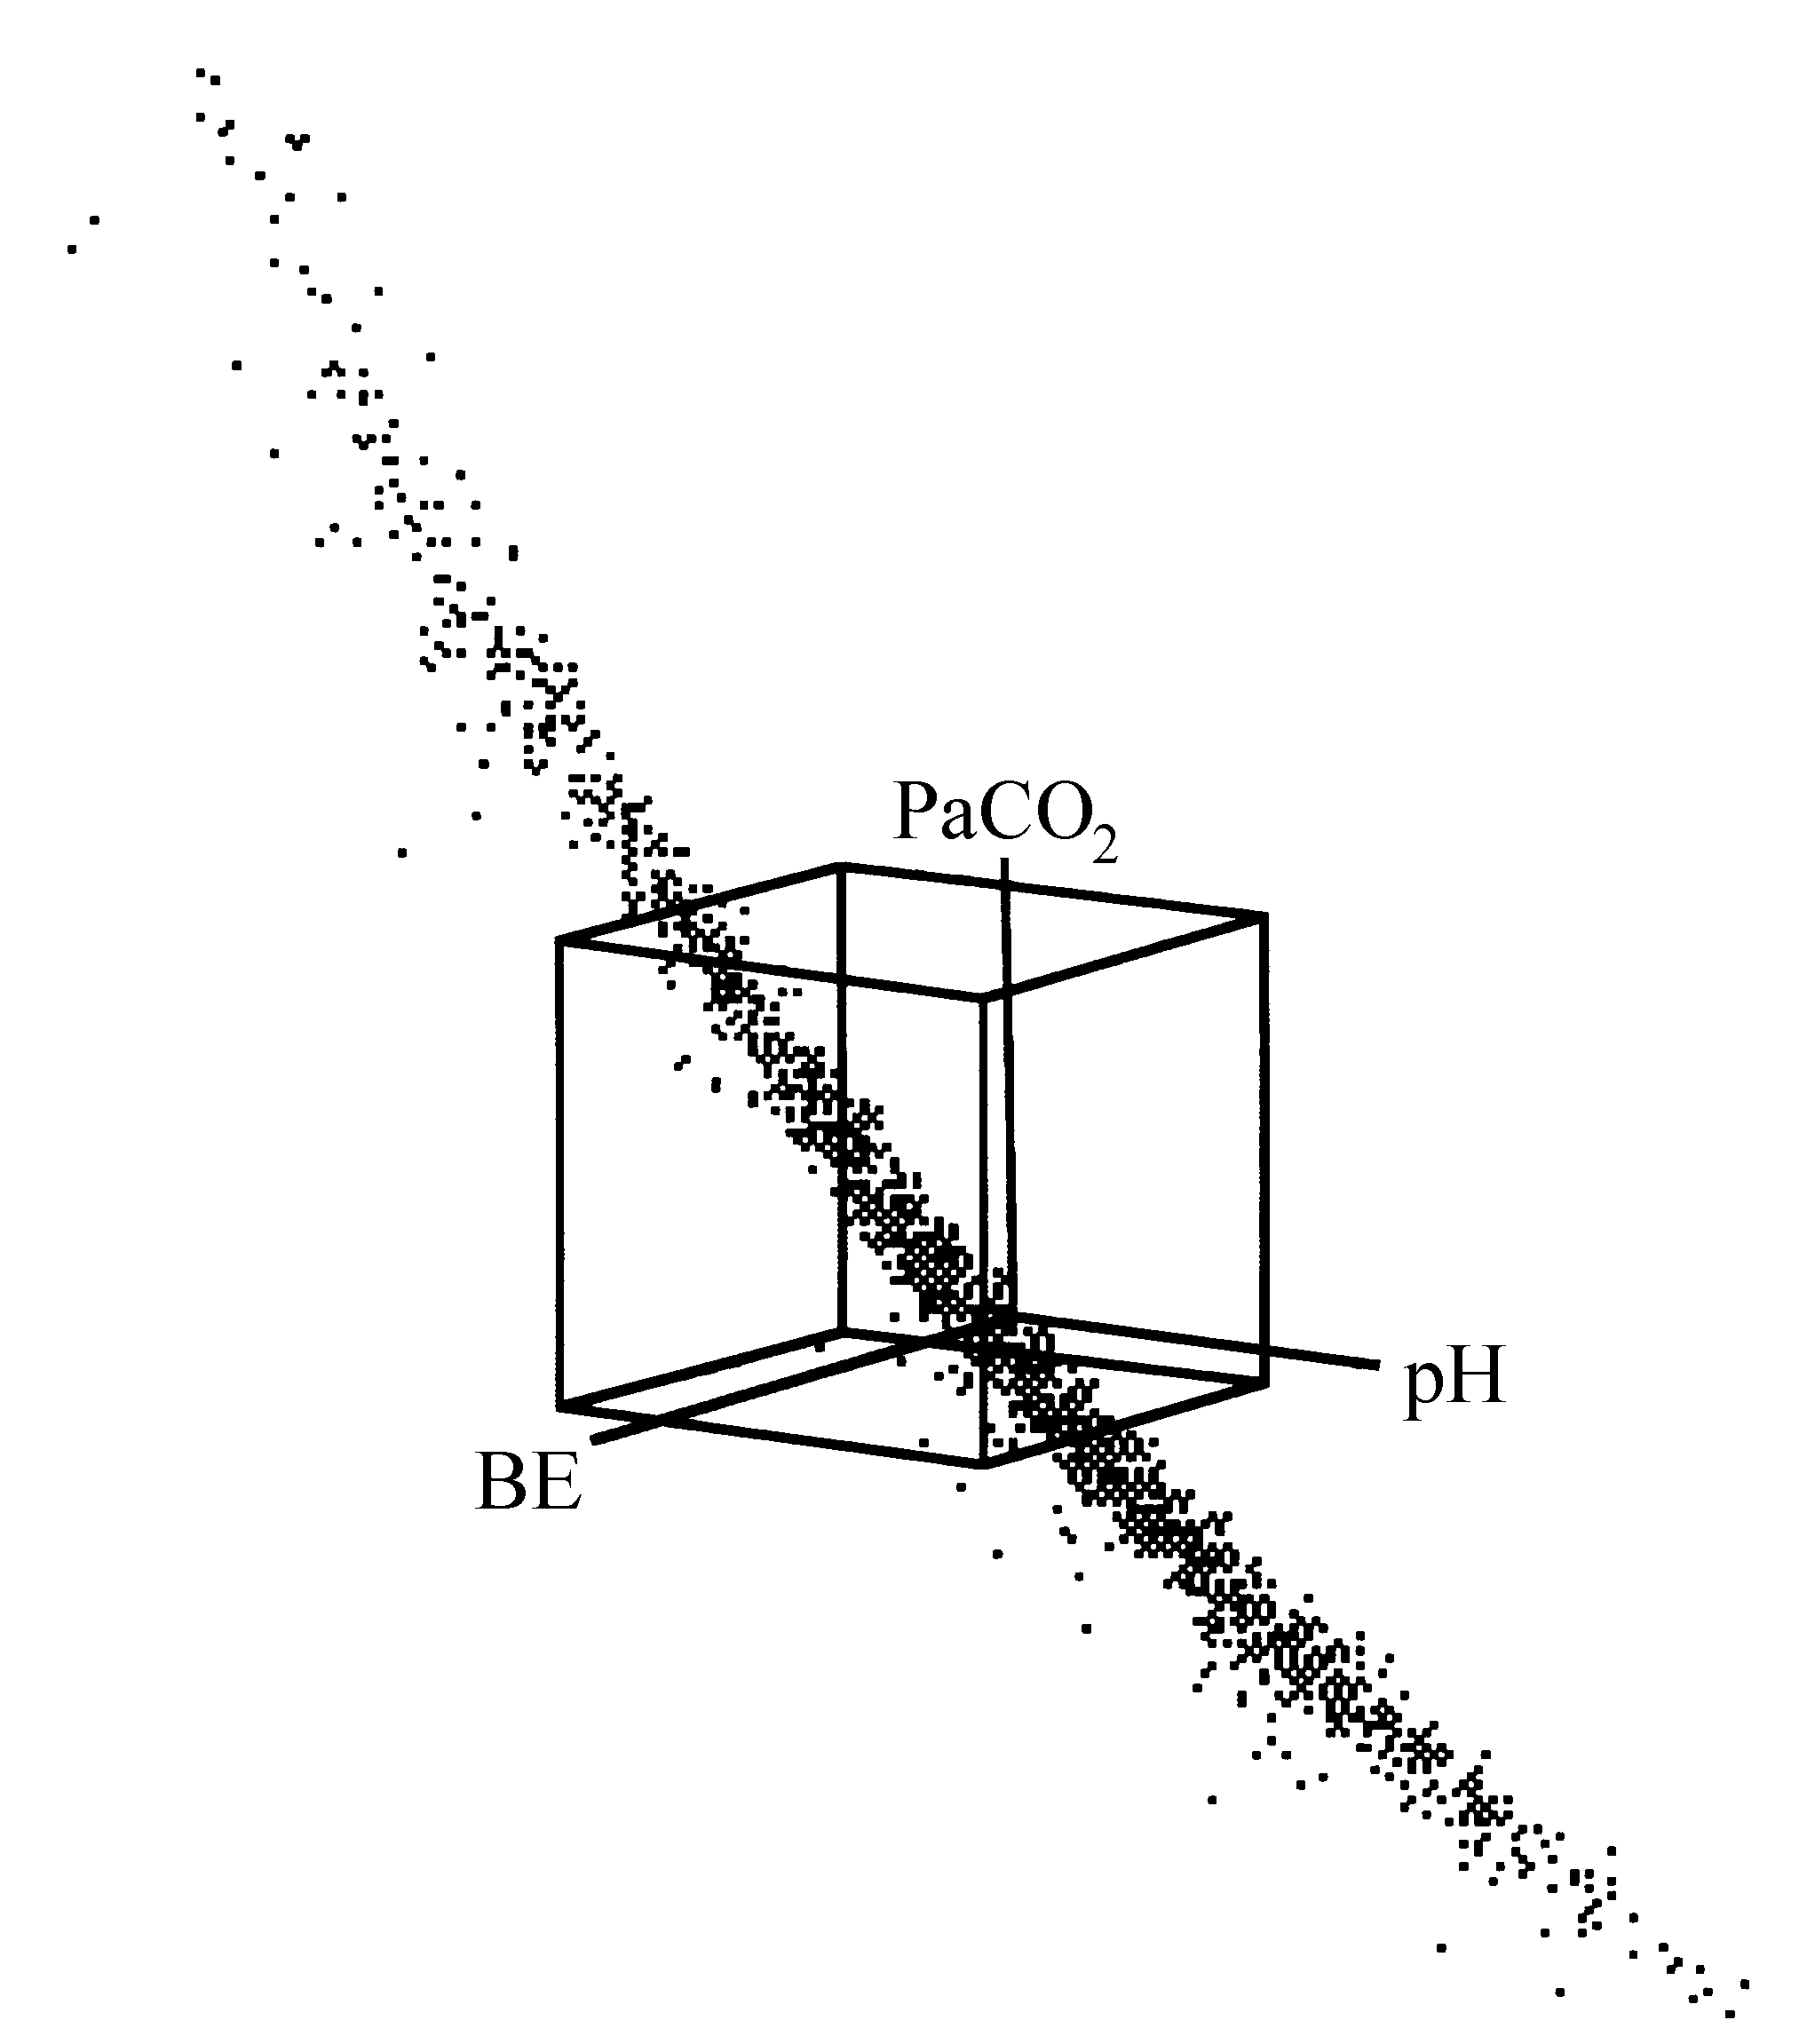
\includegraphics[width=0.8\textwidth,height=\textheight]{figures/H_02_image1.gif}

Figure 2 --1 displays such a pH, \(\ce{PaCO}_{2}\) and BE distribution
in three dimensions. The distribution is rotated in such a way that the
curved plane of measurements can be easily viewed. The cube in the
middle is the volume in three dimensions that represents the standard
reference volume, as built from the three standard univariate 95\%
reference intervals for pH, \(\ce{PaCO}_{2}\) and BE of Table 2 --1.

Having observed that the relationship between the arterial acid-base
variables (both for combinations of pH, \(\ce{PaCO}_{2}\) and BE and pH,
log \(\ce{PaCO}_{2}\) and log a{[}\(\ce{HCO}_{3}^{-}\){]}) is an almost
linear one, the goal is to arrive at a mathematical description of this
relationship and to investigate its departure from linearity. The
mathematical technique to be used for such an investigation is a
principal component analysis (PCA). PCA is a multivariate statistical
technique for the compression of large data matrices {[}4, 5{]}. In this
chapter, the results of a PCA of several distributions of acid-base
data, coming from various ICUs, are described.

\hypertarget{materials-and-methods}{%
\section{Materials and methods}\label{materials-and-methods}}

\hypertarget{patient-data}{%
\subsection{Patient data}\label{patient-data}}

Six acid-base data sets from four different intensive care units were
submitted to PCA. Data set \emph{AZRbe} contains 1500 unselected
combinations of pH, \(\ce{PaCO}_{2}\) and BE values from patients of the
respiratory ICU of the Dijkzigt academic hospital, Rotterdam, The
Netherlands. The term \emph{unselected} means that no specific selection
criteria were applied. In fact, all data sets are constructed by
sampling the acid-base data as consecutively measured in the respective
clinical laboratories. Data set \emph{OLVGbe} contains 1500 unselected
combinations of pH, \(\ce{PaCO}_{2}\) and BE values from patients of the
general ICU of the OLVG hospital, Amsterdam, The Netherlands. Data set
\emph{OLVGab} comprises the 1500 combinations of pH, log
\(\ce{PaCO}_{2}\) and log a{[}\(\ce{HCO}_{3}^{-}\){]} values from the
same patients as the \emph{OLVGbe} data set. Data set \emph{SKZbe}
contains 1500 combinations of pH, \(\ce{PaCO}_{2}\) and BE values from
patients of the neonatal ICU of the Sophia Children's hospital,
Rotterdam, The Netherlands. The data set is composed of equal numbers of
data in three age groups: new-borns younger than five days, infants
between five days and one month of age, and infants aged between one
month and one year. Data set \emph{ELIbe} contains 1500 unselected
combinations of pH, \(\ce{PaCO}_{2}\) and BE values from the general ICU
of the St.~Elisabeth hospital, Tilburg, The Netherlands. Data set
\emph{ELIab} comprises the 1500 combinations of pH, log
\(\ce{PaCO}_{2}\) and log a{[}\(\ce{HCO}_{3}^{-}\){]} from the same
patients as the \emph{ELIbe} data set.

\hypertarget{standardisation}{%
\subsection{Standardisation}\label{standardisation}}

Prior to the principal component analysis of an acid-base data set, each
variable in the data set was standardised with fixed means and standard
deviations according to:

\(z_{i} = \frac{x_{i} - m}{s}\), \emph{i} = 1,...,\emph{N} (2--1)

where \emph{m} and \emph{s} are, respectively, the mean and standard
deviation for the respective acid-base variables as presented in Table 2
--1, while \emph{N} is the total number of cases in the data set. The
\emph{z\textsubscript{i}-}values are therefore the deviations from the
mean \emph{m}, measured in units of the corresponding standard deviation
\emph{s}.

\hypertarget{principal-component-analysis}{%
\subsection{Principal component
analysis}\label{principal-component-analysis}}

The standardised data sets were then subjected to PCA. PCA is a
mathematical transformation that enables the reduction of the number of
variables in a multivariate data set whilst preserving as much of the
original information as possible {[}4, 5{]}. Assuming a multivariate
data set with \emph{p} variables (\emph{x\textsubscript{1}},
\emph{x\textsubscript{2}},..., \emph{x\textsubscript{p}}), PCA finds a
new set of derived variables (\emph{z\textsubscript{1}},
\emph{z\textsubscript{2}},...,\emph{z\textsubscript{p}}) that are linear
functions of \emph{x\textsubscript{1}}, \emph{x\textsubscript{2}},...,
\emph{x\textsubscript{p}} with the following properties:

\begin{itemize}
\item
  \emph{z\textsubscript{1}} has maximum possible variance among all
  possible linear functions of \emph{x\textsubscript{1}},
  \emph{x\textsubscript{2}},..., \emph{x\textsubscript{p}}.
\item
  \emph{z\textsubscript{k}} has maximum possible variance among all
  possible linear functions of \emph{x\textsubscript{1}},
  \emph{x\textsubscript{2}},...,\emph{x\textsubscript{p}}, subject to
  z\emph{\textsubscript{k}} being uncorrelated with
  \emph{z\textsubscript{1}},
  \emph{z\textsubscript{2}},...\emph{z\textsubscript{k-1}}, for 2 ≤
  \emph{k} ≤ \emph{p} {[}4{]}.
\end{itemize}

The derived variables \emph{z\textsubscript{1}},
\emph{z\textsubscript{2}},...,\emph{z\textsubscript{p}} are called the
principal components or PCs.

In linear algebraic terms, PCs are determined with an eigenvalue
transformation of the variance-covariance matrix as derived from the
multivariate data set. For a set of \emph{N} vectors
\textbf{x}\emph{\textsubscript{i}} (\emph{i} = 1,..., \emph{N}) in a
\emph{p}-dimensional data set, the variance-covariance matrix V is
defined as:

\[V = \frac{\sum_{i = 1}^{N}{(x_{i} - m)(x_{i} - m)^{T}}}{N(N - 1)}\]
(2--2)

where \textbf{m} is the vector of the mean of the set
\textbf{x}\emph{\textsubscript{i}} (\emph{i} = 1,..., \emph{N}) and the
superscript \textsc{t} indicates transposition of a vector, in the
convention that an untransposed vector is a column vector. The
eigenvalue transformation yields a transformation matrix U, which
transforms the original vectors \textbf{x} into vectors \textbf{y},
according to \textbf{y} = U \textbf{x}, such that the
variance-covariance matrix W = UVU\textsuperscript{T} of the transformed
vectors \textbf{y} is a diagonal matrix. If U is constrained to be a
unitary matrix, the component variances of the transformed vectors
\textbf{y} appear as eigenvalues (λ) in the analysis and are found as
the diagonal elements of W.

Since the eigenvalue transformation diagonalises the variance-covariance
matrix, the total variance in the set of original vectors \textbf{x} is
decomposed into \emph{p} orthogonal directions. Thus, for a set of
\emph{p}-dimensional vectors \textbf{x} for which it is observed that
most of the variance is confined to a subspace of dimension \emph{l}
\textless{} \emph{p}, it is expected that the components 1 through
\emph{l} of the transformed vectors \textbf{y} contain most of the
useful information. The components \emph{l} +1 through \emph{p} have
only a small variance, and thus convey (almost) no information. In the
present situation, \emph{p} = 3 and due to the (almost) linear
relationships between the variables in the standardised data sets, it is
expected that \emph{l~}=~2.

\hypertarget{results}{%
\section{Results}\label{results}}

Table 2 --2 presents the results of the principal component analysis of
each data set. The eigenvalues λ are shown for each of the three
principal components (hereafter referred to as PC1, PC2 and PC3). The
eigenvalues λ explain the contribution of each of the principal
component to the total variance in the data set prior to PCA. For
instance, in the \emph{AZRbe} data set, PC1, PC2 and PC3 explain
62.37\%, 36.91\% and 0.71\% of the total variance in the initial data
set, respectively. From Table 2 --2 it can be concluded that for each
data set, the percentage of variance explained by the third principal
component (PC3) is only small compared to the variance explained by the
first two principal components (PC1 and PC2) together. The explained
variance by PC1 and PC2 for each data set is more than 99\%. The data
sets \emph{OLVGab} and \emph{ELIab} show the smallest explained variance
by PC3; 0.03\% and 0.09\%, respectively. This is not surprising since
these data sets consist of pH, log \(\ce{PaCO}_{2}\) and log
a{[}\(\ce{HCO}_{3}^{-}\){]} values and these variables are linearly
related according to the Henderson-Hasselbalch equation (see Chapter
Error: Reference source not found) {[}1{]}.

For each data set, a matrix U can be built from the three separate
normalised eigenvectors ε, which are used to calculate the associated
principal component values from a combination of standardised original
acid-base values. Table 2 --3 shows the normalised eigenvectors ε of
each principal component for all data sets. With the matrices U, new
trivariate distributions of principal component values were calculated
from the original standardised acid-base data sets.

Table 2 --4 presents the characteristics of the resulting principal
component value distributions. For each data set, the standard deviation
of the PC3 distribution is small compared to the standard deviations of
the PC1 and PC2 distributions. Data set \emph{OLVGab} and \emph{ELIab}
have the smallest standard deviations for the third principal component
value distribution: 0.097 and 0.178, respectively. This is in accordance
with the results presented in Table 2 --2.

Since for each data set the amount of explained variance is more than
99\% when only PC1 and PC2 are considered, there is no significant loss
of information when the acid-base values are projected onto the plane
spanned by PC1 and PC2. Hence, any quantitative analysis based on PC1
and PC2 addresses the complete acid-base status. In Figure 2 --2,
scatterplots of PC2 versus PC1 are shown for all data sets.

Since the plane of measurements in case of a pH, \(\ce{PaCO}_{2}\) and
BE data set is slightly curved (see Figure 2 --1), it is interesting to
investigate the effect of the curvature on the distribution of PC3
values. Therefore, the PC3 distribution characteristics of two data sets
were investigated. This was done by constructing box-whisker plots of
groups of PC3 values that are increasingly further away from the
bivariate PC1-PC2 mean. As a cut-off point, a distance of 1 standard
deviation score was chosen with a maximum of 10, yielding 11 groups of
data. A box-whisker plot provides a graphical representation of the
distribution of values in a given data set. The outer top and bottom
horizontal lines of the box-whisker plots indicate the
95\textsuperscript{th} and 5\textsuperscript{th} percentiles of a
distribution, respectively. The top and bottom horizontal lines
enclosing the box denote the 75\textsuperscript{th} and the
25\textsuperscript{th} percentile, respectively. The horizontal line
inside the box denotes the median.


\includegraphics[width=5.41944in,height=4.44722in]{figures/H_02_image2.png}

Figure 2 --3 shows the box-whisker plots for the \emph{OLVGbe} data set.
In Figure 2 --4 the box-whisker plots are shown for the \emph{OLVGab}
data set. Comparing both figures, it is apparent that with increasing
distance from the mean in the plane spanned by the first two principal
components PC1 and PC2, the variance in the PC3 distribution increases
for data set \emph{OLVGbe}, while the variance in the PC3 distribution
of data set \emph{OLVGab} remains the same for all distance strata.
These figures illustrate the slight curvature of a PCA transformed pH,
\(\ce{PaCO}_{2}\) and BE data set which is absent in a PCA transformed
pH, log PaCO2 and log a{[}\(\ce{HCO}_{3}^{-}\){]} dataset.

Figure 2 --5 presents a histogram of the 1500 calculated PC3 values of
the transformed \emph{OLVGab} distribution. The straight line in the
normal probability plot in the upper part of Figure 2 --5 indicates that
the 1500 PC3 values are normally distributed. This was confirmed with a
Kolmogorov-Smirnov distribution fit test (D\textsubscript{max} of 0.03
with a \emph{p}-value of 0.118). Since these PC3 values are normally
distributed, a parametric 95\% reference interval may be derived from
this distribution as \emph{m} ± 2\emph{s}, resulting in a reference
range of -0.472~to -0.092. The calculated PC3 value of a pH, log
\(\ce{PaCO}_{2}\), log a{[}\(\ce{HCO}_{3}^{-}\){]} combination from an
ICU patient of the OLVG hospital, transformed with the corresponding
eigenvectors of Table 2 --3, will have a probability of 95\% of being
located within this interval. A similar analysis, however, on the 1500
PC3 values of the transformed data set \emph{ELIab} showed a bimodal
distribution of PC3 values (Figure 2 --6). Consequently, the
distribution was found to be significantly deviating from a normal
distribution (D\textsubscript{max} of 0.263 with a \emph{p}-value
\textless{} 0.01).

\hypertarget{discussion}{%
\section{Discussion}\label{discussion}}

In 1979, Madias \emph{et al}. {[}6{]} already noted that, when
evaluating an acid-base status, it is illogical and fundamentally wrong
to use pH, \(\ce{PaCO}_{2}\) as well as a{[}\(\ce{HCO}_{3}^{-}\){]},
while only two of these three variables are free to change
independently. He proposed to evaluate acid-base disorders with only two
of the three basic acid-base variables. This means, however, that
clinicians are deprived of one of the three variables on which the
interpretation of the acid-base status is traditionally

In this chapter, a solution is proposed that allows a quantitative
analysis of all three basic acid-base variables while being faithful to
the interdependence between them. A multivariate statistical technique
called principal component analysis (PCA) was used to reduce the
dimensionality of large trivariate distributions of acid-base variables.
Results show that the acid-base status can be faithfully represented in
a principal component subspace defined by the principal components PC1
and PC2, without significant loss of information. The distortion,
measured as a percentage of variance not represented, is shown to be
less than 0.7\% for all the data sets investigated. The (small)
percentage of explained variance by PC3 in data sets of pH, log
\(\ce{PaCO}_{2}\) and log a{[}\(\ce{HCO}_{3}^{-}\){]} (data sets
\emph{OLVGab} and \emph{ELIab}) may be attributed to rounding effects
and analytical imprecision. For the other data sets, consisting of pH,
\(\ce{PaCO}_{2}\) and BE values, the curvature of the plane of
measurements is an extra source of variance resulting in larger
percentages of variance explained by PC3. However, this source of
variance is only minor and for each data set it is therefore justified
that quantitative analyses of acid-base disorders be based on PC1 and
PC2 values after a PCA transformation, rather than on the original
acid-base values. Furthermore, projection of the original points onto
the PC1-PC2 subspace is (almost) distortionless. In Chapter Error:
Reference source not found, this characteristic is used to define a
sound way to graphically represent all three acid-base variables in a
single two-dimensional representation.

The minor variance in PC3 may also serve as a plausibility check for
acid-base laboratory values; each transformed combination of pH,
\(\ce{PaCO}_{2}\) and a{[}\(\ce{HCO}_{3}^{-}\){]}/BE must lead to a
small PC3 value. For a pH, log \(\ce{PaCO}_{2}\) and log
a{[}\(\ce{HCO}_{3}^{-}\){]} data set, PC3 must be within the 95\%
reference interval for PC3 as obtained from the PC3 values after PCA of
an acid-base data set. For instance, the 95\% reference interval for PC3
of the \emph{OLVGab} data set was found to be -0.472 to 0.092. If a
transformed combination of acid-base measurements is not within the
interval, then it may be concluded that this specific combination of pH,
PaCO­\textsubscript{2} and a{[}\(\ce{HCO}_{3}^{-}\){]} is not valid.
Note that the interval is not equally centred around zero. From the
definition of PCA one would expect that, when calculated means and
standard deviations are used, the mean value for all principal component
values would be zero. However, for the standardisation procedure the
fixed means and standard deviations of Table 2 --1 were used, leading to
the observation that the mean values of the principal components are
different from 0 for the various data sets, since they have different
means and variances for the original acid-base values.

Checking whether the PC3 value of a transformed acid-base observation is
within the 95\% reference interval is only possible for data sets of pH,
log \(\ce{PaCO}_{2}\) and log a{[}\(\ce{HCO}_{3}^{-}\){]}, since the
variance in PC3 is independent of the distance of an observation to the
PC1-PC2 bivariate mean (see Figure 2 --6). Observations in a data set of
pH, PaCO­­\textsubscript{2} and BE are located on a slightly curved
plane of measurements, resulting in the effect that with increasing
distances from the PC1-PC2 bivariate mean, the variance in PC3 increases
(see Figure 2 --3). To check the plausibility of a transformed pH,
\(\ce{PaCO}_{2}\) and BE combination one could either use the variance
in PC3 as found for data with distances larger than or equal to 10
standard deviations scores (≥ 10), or use the variance in PC3 in the
associated distance group.

One could argue that the relationship between the acid-base variables
could be described by studying the formula used in acid-base analysers
to calculate a{[}\(\ce{HCO}_{3}^{-}\){]} or BE from measured pH,
\(\ce{PaCO}_{2}\) and haemoglobin. The advantage of the approach
presented in this chapter, however, is that no prior knowledge is needed
about the formula with which the a{[}\(\ce{HCO}_{3}^{-}\){]} or the BE
are calculated. The method, therefore, adapts itself to the instruments
used.

\hypertarget{acknowledgements}{%
\section{Acknowledgements}\label{acknowledgements}}

I am indebted to dr. R.N.M. Weijers and dr. D. Zandstra for making the
data sets \emph{OLVGbe} and \emph{OLVGab} available. Dr.~B. van der Berg
and dr. R.W. Wulkan contributed similar material: the data sets
\emph{AZRbe} and \emph{SKZbe}, respectively. Finally, dr. J.E. van
Puyenbroek and dr. B. Speelberg provided the data sets \emph{ELIbe} and
\emph{ELIab}.

\hypertarget{references-1}{%
\section{References}\label{references-1}}

1. Rose BD. Clinical Physiology of Acid-Base and Electrolyte Disorders.
4th Edition, New York: McGraw-Hill, Inc., 1994; 853.2. Astrup P,
Jörgensen K, Siggaard-Andersen O, et al.~The acid-base metabolism, a new
approach. \emph{Lancet} 1960;1035-1039.3. Gelsema ES, Leijnse B, Wulkan
RW. A multi-dimensional analysis of three chemical quantities in the
blood. \emph{Med Inform} 1991; 16:43-54.4. Jolliffe IT, Morgan BJT.
Principal component analysis and exploratory factor analysis. \emph{Stat
Meth Med Res} 1992; 1:69-95.5. Jolliffe IT. Principal Component
Analysis. New York: Springer-Verlag, 1986, \emph{Springer Series in
Statistics}; vol 12.6. Madias NE, Adroqué HJ, Horowitz GL, et al.~A
redefinition of normal acid-base equilibrium in man: Carbon dioxide
tension as a key determinant of normal plasma bicarbonate concentration.
\emph{Kidney Int} 1979; 16:612-618.

\end{document}
